The total charge accumulated by a certain device is given as function of time by $q= 18t^2-2t^4$. Find: (\emph{a}) the total charge at $t=2$; (\emph{b}) the maximum charge in $0\leq t\leq 3$ and when it occurs; (\emph{c}) the rate that charge is accumulated at $t=0.8$; (\emph{d}) sketch curves of $i$ vs $t$ and $q$ vs $t$ in $0\leq t\leq 3$  

\begin{enumerate}[leftmargin=2cm,labelsep=.5cm,label=\bfseries\alph*)]
	\item $
	\begin{aligned}[t]
	18(2^2) - 2(2^4) &= \hlbox{40\text{ C}} \\
	\end{aligned} $
	\\[.5cm]
	
	\item $
	\begin{aligned}[t]
	&q'= 36t-8t^3 \\[0.2cm]
	&36t-8t^3= 0,\; t\geq 0 \\
	&t=0,\; t=2.121 \\[0.2cm]
	&q_{max} = \hlbox{40.5\text{ C at } 2.121\qw{\second}} \\
	\end{aligned} $
	\\[.5cm]
	
	\item $
	\begin{aligned}[t]
	&q'= 36t-8t^3 \\
	&36(0.8)-8(0.8^3) = \hlbox{24.704\text{ C/s}}\\
	\end{aligned} $
	\\[.5cm]
	
	\item $q$ vs $t$:
	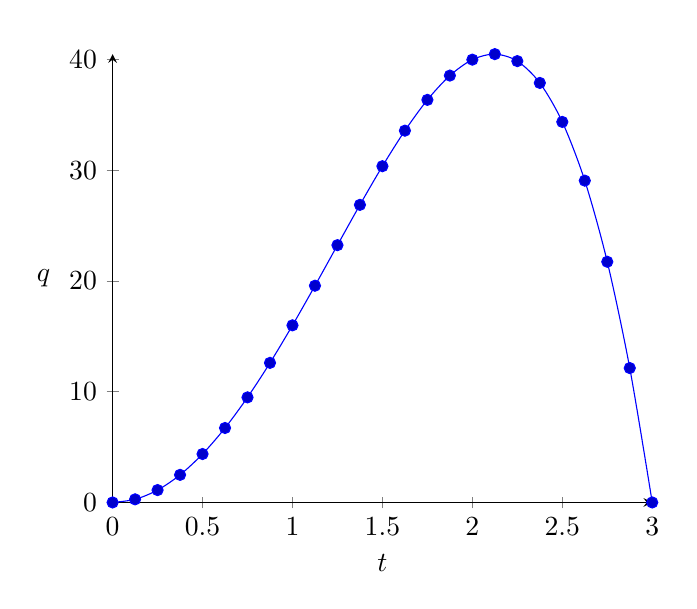
\begin{tikzpicture}[level/.style={sibling distance=50mm/#1},baseline={([yshift=.5em] current bounding box.north)}]
	\begin{axis}[axis lines=left,xlabel=$t$,ylabel=$q$, ylabel style={rotate=-90}]
		\addplot+[smooth,domain=0:3] {18*x^2 - 2*x^4};
	\end{axis}
	\end{tikzpicture} \\
	$i$ vs $t$:
	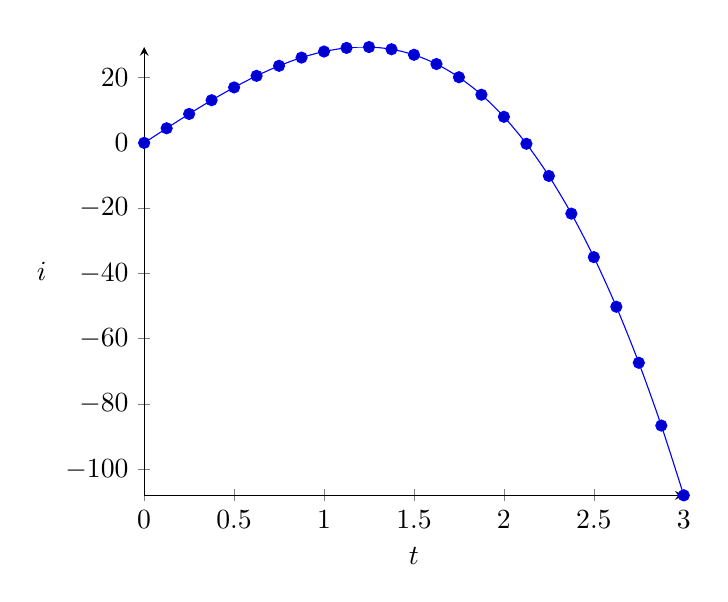
\begin{tikzpicture}[level/.style={sibling distance=50mm/#1},baseline={([yshift=.5em] current bounding box.north)}]
	\begin{axis}[axis lines=left,xlabel=$t$,ylabel=$i$, ylabel style={rotate=-90}]
	\addplot+[smooth,domain=0:3] {36*x - 8*x^3};
	\end{axis}
	\end{tikzpicture}
\end{enumerate}